\documentclass[11pt, a4paper]{article}
\usepackage[top=3cm,bottom=3cm,left=2.75cm,right=2cm]{geometry}
\usepackage{graphicx}
\usepackage[latin1]{inputenc}
\usepackage[spanish]{babel}
\usepackage{amsmath}

\begin{document}


\begin{figure}[t] %[h] para here [b] para bottom [t] para top
\centering

\includegraphics[width=80pt]{./logo.jpg}
\end{figure}


\begin{center}


\LARGE{UNIVERSIDAD DE BUENOS AIRES}
\Large{FACULTAD DE CIENCIAS EXACTAS Y NATURALES\\
DEPARTAMENTO DE COMPUTACI\'ON\\
\vspace{1.5cm}
ORGANIZACI\'ON DEL COMPUTADOR II\\
Segundo Cuatrimestre de 2009}

\vskip 50pt
\textbf{\Large{Procesamiento de Im\'agenes para la Detecci\'on de Bordes}}

\end{center}

\vskip 30pt

\begin{center}
\begin{tabular}{|lcl|}
\hline Integrante & LU & Correo electr\'onico \\
\hline Bianchi, Mariano & 92/08 & \texttt{bianchi-mariano@hotmail.com}\\
Brusco, Pablo & 527/08 & \texttt{pablo.brusco@gmail.com} \\
Di Pietro, Carlos Augusto Lyon & 126/08 & \texttt{cdipietro@dc.uba.ar}\\
\hline
\end{tabular}

\vspace{20 pt}

Grupo : PUNPCKHQDQ

\end{center}

\vskip 60pt

{\small
\flushleft{\textbf{Resumen}}\\
La detecci\'on de bordes es una herramienta sumamente utilizada en el procesamiento de im\'agenes, la cual permite dar mayor importancia a ciertos datos como son las l\'neas, los contornos y trazos de las mismas en detrimento de otros detalles como pueden ser matices sutiles y l\'ineas muy finas. La idea del presente trabajo es lograr implementar algoritmos de detecci\'on de bordes de im\'agenes vali\'endose para ello de los operadores m\'as comunes para tal fin. Estos son los operadores de Sobel, Prewitt y Roberts.\\
Como paso ulterior se buscar\'a comparar los resultados obtenidos con funciones an\'alogas implementadas en la librer\'ia estandar de c\'odigo abierto OpenCV. Los aspectos a comparar ser\'an tanto la calidad de resultados como el tiempo de
procesamiento medido en ciclos de reloj.\\

\vspace{22 pt}

\flushleft{\textbf{Palabras clave}}\\
Deteccion de bordes, Sobel, Roberts, Prewitt, convoluci\'on, imagenes, Lena , OpenCV.
}


\newpage



\section{Introducci\'on}

\paragraph{}
La detecci\'on de bordes es una herramienta muy utilizada dentro del \'area del procesamiento de im\'agenes. Esto se debe a que los m\'etodos de detecci\'on de bordes filtran la informaci\'on inecesaria preservando las caracter\'isticas fundamentales de la imagen, dejando por resultado una imagen que contiene toda la informaci\'on relevante de la original como son los contornos, lineas y trazos de la imagen.

\paragraph{}
En este sentido, para que un m\'etodo sea capaz de detectar un borde en necesario definir de manera no ambigua que se considera un borde. De este modo, si consideramos al pixel como la menor unidad de imagen, podr\'iamos decir que un borde se caracteriza por ser un cambio abrupto en la intensidad de pixeles vecinos.\\
Abstrayendo esta idea al plano matem\'atico, podemos caracterizar a la intensidad de los pixeles que componen la imagen como una funci\'on continua cuya representaci\'on es una curva suave salvo por picos en los cuales se produce un salto en la intensidad. Luego, para detectar un borde lo que se busca determinar son los puntos que se corresponden con los saltos de intensidad en una imagen.\\
Para ello se emplea una de las herramientas m\'as utilizadas que es el vector gradiente, el cual gr\'aficamente siempre apunta en direcci\'on a la mayor variaci\'on de la funci\'on. En nuestro an\'alisis particular, el vector gradiente act\'ua como indicador de la direcci\'on en la cual se produce la mayor variaci\'on de intensidad entre un pixel y cualquiera de sus vecinos.

\paragraph{}
Lo esperable es poder cuantificar esa m\'axima variaci\'on de intensidad entre los pixeles, razon por la cual, para cada pixel se desea determinar la norma de su vector gradiente. Se sabe por definici\'on del vector gradiente que:


$$
\nabla I = \left[ \begin{array}{l}
\vspace{11 pt}
I_x\\
I_y
\end{array}
\right]
= \left[ \begin{array}{l}
\vspace{11 pt}
\frac{\sigma I}{\sigma x}\\
\frac{\sigma I}{\sigma y}
\end{array}
\right]
$$



Luego, la norma del vector gradiente queda caracterizada por la expresi\'on:

\begin{equation}
||\nabla I|| = \sqrt{I_x ^{2}+ I_y^{2}}
\end{equation}



No obstante, para reducir la complejidad computacional, en este trabajo se opt\'o por aproximar esta norma mediante la suma de los m\'odulos de las derivadas parciales

\begin{equation}
||\nabla I|| \approx |I_x| + |I_y|
\end{equation}


En consecuencia, para calcular el gradiente de una imagen, se debe realizar previamente el c\'alculo de las derivadas parciales en cada pixel.
La forma optada en este trabajo pr\'actico para calcular dichas derivadas es mediante la aplicaci\'on de operadores dobles o de dos etapas. Los operadores utilizados, fueron los operadores de Sobel, Prewitt y Roberts. Estos operadores se caracterizan por realizar la detecci\'on de bordes en dos pasos. En el primero se buscan los bordes horizontales utilizando la m\'ascara que corresponde a la derivada parcial en X a cada pixel de la imagen. Seguidamente, y de forma an\'aloga, se buscan los bordes verticales utilizando la m\'ascara que corresponde a la derivada parcial en Y. Finalmente, para obtener todos los bordes de la imagen se suman los bordes horizontales y verticales obtenidos en el paso previo.


\paragraph{}
El objetivo de este trabajo pr\'actico es implementar un programa capaz de detectar los bordes de una imagen mediante el uso de los m\'etodos anteriormente descriptos. Se pretende que la interfaz del mismo se desarrolle en lenguaje C y que las funciones de detecci\'on de bordes se encuentren desarrolladas en lenguaje assembler.
Para la implementacion de la interfaz, se cuenta con las funciones incluidas en la librer\'ia de codigo abierto OpenCV. Esta librer\'ia provee, entre otras cosas, funciones que simplifican la carga, copia y salvado de im\'agenes, asi como tambi\'en otras funcionalidades necesarias para la realizaci\'on de este trabajo. En particular, provee tambien la funci\'on cvSobel, la cual realiza la detecci\'on de bordes de una imagen usando el operador de Sobel.
Una vez desarrollado el programa, se pretende poder comparar los m\'etodos implementados en este trabajo, con los m\'etodos provenientes de la librer\'ia de codigo abierto OpenCV. Para dicha comparaci\'on, en el caso del operador de Sobel, se har\'a uso de la funcion cvSobel anteriormente mencionada. Adem\'as, nos interesa cuantificar, la diferencia de velocidad entre las implementaciones de la librer\'ia y las del presente trabajo en funci\'on de la cantidad de ciclos de reloj necesarios para procesar una imagen.

En lo que respecta al trabajo final, el programa desarrollado es capaz de aplicar el m\'etodo de detecci\'on de bordes usando todos los operadores mencionados, dando la posibilidad de hallar bordes de toda una imagen en sus dos direcciones; mientras que en caso particular del operador de Sobel, tambi\'en brinda la opci\'on de calcular los bordes horizontales y verticales, no as\'i para los operadores de Prewitt y Roberts.

\newpage

\section{Desarrollo}

\subsection{Primera aproximaci\'on}
\paragraph{}
Para comenzar a realizar este trabajo pr\'actico lo primero que se hizo, a modo de prueba y al igual que en el trabajo anterior, fue realizar simplemente un recorrido de la imagen copiando pixel por pixel, obteniendo as\'i una copia fiel de la imagen fuente en la imagen destino. De esta modo, se aseguraba que la forma de recorrer la imagen fuese la correcta. Esto se realiz\'o porque no resultaba trivial recorrer una im\'agen de ancho m\'ultiplo de 16 de a menos pixeles.

\subsection{Implementaci\'on}
\paragraph*{}
Ya habi\'endose realizado suficientes pruebas se procedi\'o a implemetar el algoritmo deseado. Como primer paso se implement\'o la intrfaz del mismo en lenguaje C, de modo de que al ejecutar el programa por consola, este pudiera recibir como par\'ametro la imagen a procesar, asi como tambi\'en el tipo de filtro a aplicar conforme a lo pedido en el enunciado del presente trabajo.
Seguidamente se pas\'o a analizar la forma en la cu\'al se implementar\'ia cada m\'etodo. Se comenz\'o por el m\'etodo de Sobel, ya que si este m\'etodo se implementaba correctamente, el resto pod\'ia resolverse de manera an\'aloga (o en su defecto de manera muy similar), cambiando en cada caso la m\'ascara a aplicar.
De este modo, se busc\'o que el algoritmo de Sobel fuera recorriendo la imagen y aplicara a cada pixel se aplicaba la m\'ascara correspondiente, es decir la matriz de 3x3 con los valores correspondientes al operador de Sobel . Esta aplicaci\'on se realizaba de la siguiente manera: una vez posicionados sobre el pixel al cual se le quer\'ia calcular la derivada, se tomaba una matriz de 3x3 centrada en dicho pixel (pixeles de la imagen fuente). A continuaci\'on, se multiplicaba cada pixel contiguo al que se buscaba derivar por su correspondiente en la matriz del operador, al tiempo que se iba sumando estos resultados en un acumulador.
Ahora bien, podr\'ia pasar que el valor obtenido fuera mayor o menor al rango de valores admisibles por la escala monocrom\'tica. Es decir, podr\'ia darse el caso de que el resultado de aplicar la m\'ascara a un pixel fuera mayor a 255 (blanco absoluto) o menor a cero (negro absoluto). Para subsanar esta situaci\'on, se implement\'o un algoritmo que neutralizara la aritm\'etica por desborde y emulara una aritm\'etica saturada. Este algoritmo, implementado como una macro de assembler, comparaba el resultado con 0 y con 255, y de acuerdo a si el valor resultante era mayor que 255 o menor que 0, se le reasignaba arbitrariamente los valores 255 o 0 respectivamente.\\
Finalmente, una vez obtenido el resultado, se pasaba a guardar el pixel procesado al pixel an\'alogo en la imagen destino, y se proced\'ia a procesar el pixel siguiente con el cuidado de pasar a la fila siguiente en caso de haber recorrido el el ancho de la imagen propiamente dicha, evitando de este modo, procesar los p\'ixeles de relleno que incorporan los algoritmos de carga de im\'agenes de la librer\'ia OpenCV con el fin de aumentar el hitrate de cache. Este procedimiento se repeti\'ia iterativamente hasta haberse recorrido todas las filas de la imagen, y consecuentemente cada uno de sus p\'ixeles.

\paragraph{}
A modo de comentario, cabe aclarar que, como la m\'ascara que se aplica es de 3x3, y la transformaci\'on se aplica sobre el pixel en el cual se centra dicha m\'ascara, es l\'ogico notar que los pixeles pegados a los cuatro bordes de la imagen fuente no se van a procesar. La misma situaci\'on ocurre con el m\'etodo de Prewitt. En cambio en el operador de Roberts, al ser de 2x2, se pierden nada m\'as que dos bordes. Fue decisi\'on del grupo no rellenar estos p\'ixeles bordes con ning\'un valor.

\paragraph{}
La implementaci\'on de los dem\'as m\'etodos fue an\'aloga a la realizada anteriormente, con la \'unica diferencia de que en cada caso se variaban los valores y el tama\~no de las m\'ascaras segun dependiera.

\paragraph{}
Una vez realizada la implementaci\'on para Sobel descripta anteriormente se pas\'o a comparar los resultados arrojados por la misma, con los resultantes de la implementaci\'on de la librer\'ia. R\'apidamente, se pudo observar que hab\'ia algun error en la implementaci\'on realizada, ya que las im\'agenes no se parecian en absoluto. Luego de analizar el c\'odigo, fue posible advertir que cuando se realizaba un movimiento del pixel de la imagen fuente a un registro para poder ir acumulando el valor resultante, ese movimiento lo hac\'iamos a un registro de 32 bits, por lo que en vez de estar cargando el valor de un \'unico pixel de la imagen fuente, se estaban cargando cuatro pixeles juntos. Para revertir esta situaci\'on, simplemente se cambi\'o de registro, y se ultiliz\'o uno de 8 bits. Luego de este cambio, la imagen procesada por el algoritmo implementado para este trabajo qued\'o a simple vista igual a la que devolv\'ia la implementaci\'on de la librer\'ia.

\paragraph{}
Otro aspecto que se busc\'o mejorar, ya en vista de las mediciones de ciclos de reloj, fue el de intentar reducir el costo computacional del c\'aculo de la mascarar. En efecto, dado que los valores de los operadores son $\pm$1 y $\pm$2,en todos los caso, se se pas\'o a adaptar cada implementaci\'on de modo que una vez posicionados sobre el pixel de la imagen fuente, es decir, de la imagen a procesar, en un registro acumulador se fueran realizando los c\'alculos que indicaba el operador por medio de la suma y resta de los valores de los p\'ixeles vecinos, o eventualmente la suma o resta de alg\'un valor shifteado a izquierda seg\'un correspondiese.
A modo de ejemplo, para el caso del operador de Sobel en el eje X, suponiendo que se estaba posicionado en el pixel a procesar, al acumulador se le restaba una vez el pixel de arriba a la izquierda, una vez el de abajo a la izquierda y se le una vez el de la izquierda shifiteado 1 vez a izquierda. Luego, se le sumaba una vez el de arriba a la derecha, otra vez el de abajo a la derecha, y una vez el de la derecha tambi\'en shifteado 1 vez a izquierda.\\
Una vez obtenido el valor de aplicar la m\'ascara a cada pixel, se proced\'ia a saturar el valor y se continuaba con el algoritmo conforme a lo explicado anteriormente.

\paragraph{}
Luego de estos cambios en la implementaci\'on, se pudieron ver cambios positivos en cuanto al rendimiento del procesamiento de las im\'agenes. Asimismo, no se observaron cambios en el las im\'agenes resultantes, por lo que los resultados de las comparaciones con los resultados arrojados por la librer\'ia segu\'ian siendo los mismos.
Luego de comprobar que el cambio realizado continuaba cumpliendo los requerimientos, se procedi\'o a cambiar el resto de las implementaciones adapt\'andolas seg\'un esta nueva forma.

\paragraph*{}
Como comentario al margen, cabe decir que un benieficio a la hora de realizar estar m\'odificaciones fue el hecho de haber implementado los algoritmos de forma modular. Esto permiti\'o que lo \'unico que debiera cambiar fuera la forma en que se calculaba el pixel resultante y no la forma de recorrer la matriz.

\paragraph*{}
Finalmente resta por aclarar que, al no contar con ima\'agenes procesadas por los m\'etodos de Preitt y Roberts que sirvieran como un punto de comparaci\'on preciso para los algor\'itmos implementados en este trabajo, no quedar\'ia claro si la implementaci\'on realizada es fiable o no. De todos modos, como cada implementaci\'on se bas\'o en la del operador de Sobel para el cual s\' se tuvo puento de comparaci\'on, se puede suponer que el resultado del resto de las implementaciones es bastante acertado.


\newpage

\section{Resultados}

\subsection{Mediciones de tiempos de ejecuci\'on}
\paragraph{}
A continaci\'on se presentan los resultados de las mediciones de ciclos de reloj de la ejecuci\'on de cada uno de los algoritmos. Asimismo se presenta una tabla comparativa de las mediciones de ciclos de reloj de cvSobel y la funci\'on an\'aloga realizada en este trabajo.
Por otra parte, las im\'agenes resultantes del procesamiento de bordes, que bien podr\'ian ir en esta secci\'on del informe, se encuentran al final del mismo presentadas como anexos para favorecer su visualizaci\'n.

\paragraph{}
El criterio para obtener los resultados de esta secci\'on fue realizar unas 1000 iteraci\'ones, y quedarnos con el menor tiempo arrojado por cada una de las funciones, tanto para las realizadas en este trabajo, como para las incluidas en la librer\'ia OpenCv.

\vspace{1cm}

\begin{table}[ht] %ubicacion de la tabla
\centering %centra la tabla
\begin{tabular}{|l|r|r|r|r|r|}
\hline
M\'etodo & Roberts & Prewitt & SobelX & SobelY & SobelXY \\
\hline
TP1A & 10926996 & 11055936 & 9117708 & 7862676 & 15924036 \\
\hline
TP1B & 697272 & 2294244 & 1467132 & 1452480 & 2368380 \\
\hline
\end{tabular}

\caption{Tabla comparativa de mediciones de ciclos de reloj para cada uno de los algoritmos de detecci\'on de bordes implementados en ambos trabajos pr\'acticos} %titulo de la tabla
\label{Tiempo metodos} %con esto puedo referenciar a la tabla \ref{Tiempo metodos}
\end{table}
\vspace{30pt}

\begin{table}[ht] %ubicacion de la tabla
\centering %centra la tabla
\begin{tabular}{|l|r|r|r|}
\hline
Metodo & SobelX & SobelY & SobelXY \\
\hline
TP1A & 9117708 & 7862676 & 15924036 \\
\hline
TP1B & 1467132 & 1452480 & 2368380 \\
\hline
OpenCv & 21603888 & 19262892 & 20204124 \\
\hline



\end{tabular}

\caption{Tabla comparativa de mediciones de ciclos de reloj entre los algoritmos de deteccion de bordes basados en el operador de Sobel de la libreria OpenCV y los implementados en ambos trabajos pr\'acticos} %titulo de la tabla
\label{Tiempo comparacion} %con esto puedo referenciar a la tabla \ref{Tiempo metodos}
\end{table}


\newpage
\section{Debate}
\paragraph{}
Como podemos observar en los datos obtenidos en la secci\'on de resultados, hay una clara diferencia en los ciclos de reloj necesarios para procesar una imagen entre el m\'etodo utilizado para el TP1 y el utilizado para el presente trabajo. Esto puede deberse a varios motivos, pero el principal y m\'as trivial de todos es que gracias a haber utilizado instrucciones SSE, se pudieron procesar de a m\'as de un pixel por vez haciendo aqu\'i la mayor diferencia. Adem\'as, la saturaci\'on del valor de los pixeles se realizaba automaticamente, tambi\'en gracias a las instrucciones antes mencionadas. Por lo tanto, el tiempo necesario para procesar una imagen se ve reducido ampliamente.

\paragraph{}
No obstante, la utilizaci\'on de instrucciones SSE para la mejora de ciertos puntos de un algoritmo puede ser una desventaja. Esto se debe a que no todos los procesadores tienen el mismo set de instrucciones, por lo cu\'al un algoritmo que funcione de manera excelente en una computadora, puede no comportarse como se espera en otra o directamente no funcionar.


\section{Conclusi\'ones}

\paragraph{}
Si observamos m\'as detalladamente los datos obtenidos, podremos ver grandes diferencias entre los tiempos de ejecuci\'on de la implementaci\'on anterior (TP1) y la nueva (TP2). Esto se debe a que, gracias al haber utilizado instrucciones SSE, en cada ciclo se pudieron procesar de a varios pixeles a la vez, en contraposici\'on con el trabajo pr\'actico anterior, en el cual s\'olo se pod\'ia procesar de a un pixel por vez.

\paragraph{}
Otro punto interesante es observar como se produce la saturaci\'on de un pixel. En el trabajo anterior, para poder saturar el valor obtenido para cada pixel, se deb\'ia hacer una funci\'on aparte. Esto conllevaba a un tiempo de ejecuci\'on mayor, ya que se deb\'ian hacer algunas comparaciones y asignaciones de acuerdo a si correspond\'ia saturar a 0 o a 255.\\
En el caso de este trabajo, esto era autom\'atico, por lo cual se redujeron ampliamente los tiempos de ejecuci\'on en lo que respecta al tema de saturaci\'on. 

\paragraph{}
Como conclusi\'on final, podemos decir que conociendo mejor las virtudes de un procesador se puede mejorar a\'un m\'as el tiempo de ejecuci\'on de un algoritmo realizado en lenguaje assembler. Sin embargo, se debe conocer con detalle las m\'aquinas en donde se piensa utilizar este software ya que puede no funcionar como debe, dependiendo el hardware que se utilice.


\newpage
\section{Anexo I}
\subsection{Imagenes resultantes del procesamiento de detecci\'on de bordes}

\vspace{2cm}

\begin{figure}[ht] %[h] para here [b] para bottom [t] para top
\centering
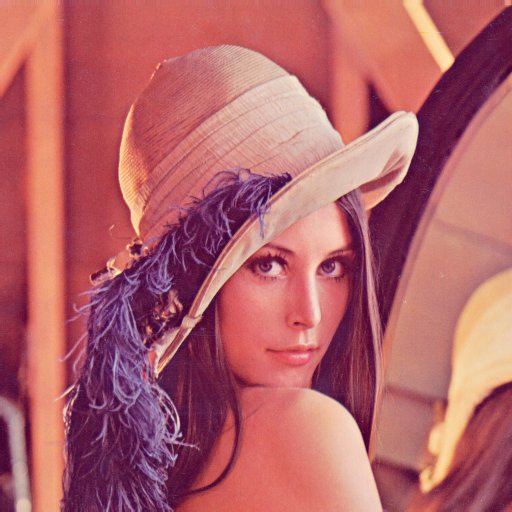
\includegraphics[scale=0.25]{lena.jpg}
\caption{Primer imagen utilizada para detecci\'on de bordes - lena.jpg}
\end{figure}

\vspace{3cm}

\begin{figure}[ht] %[h] para here [b] para bottom [t] para top
\centering
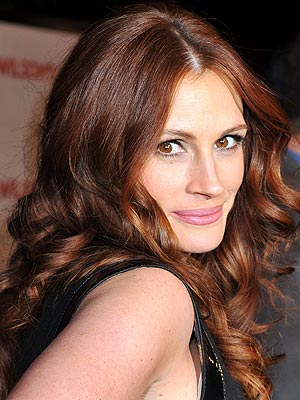
\includegraphics[scale=0.30]{roberts.jpg}\hspace{1cm}
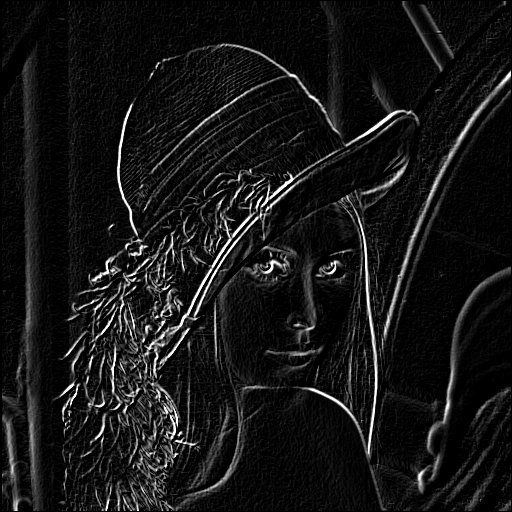
\includegraphics[scale=0.30]{prewitt.jpg}
\caption{Resultado de aplicar el operador Roberts y Prewitt para la imagen lena.jpg, respectivamente}
\end{figure}

\begin{figure}[ht] %[h] para here [b] para bottom [t] para top
\centering
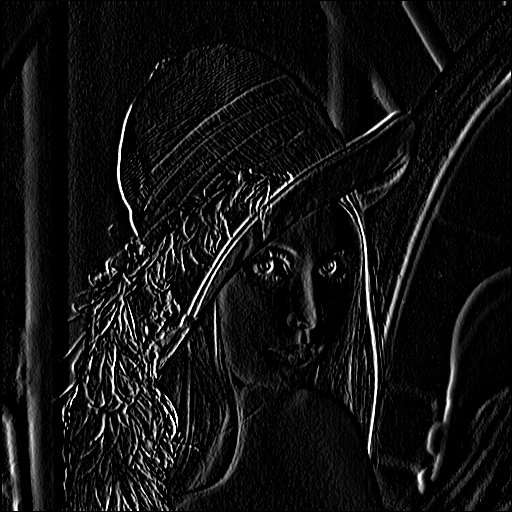
\includegraphics[scale=0.30]{sobelX.jpg}\hspace{1cm}
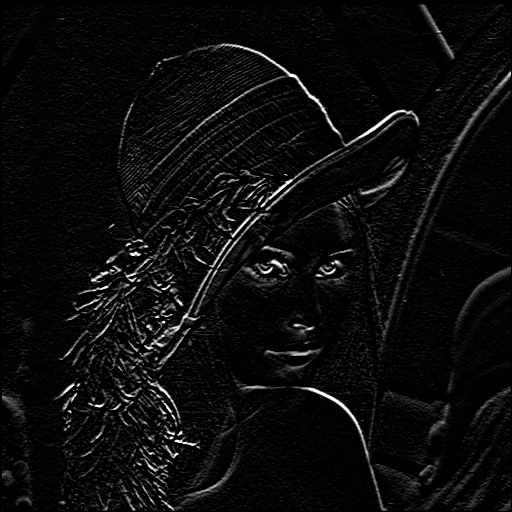
\includegraphics[scale=0.30]{sobelY.jpg}
\caption{Resultado de aplicar el operador sobelX y sobelY para la imagen lena.jpg, respectivamente}
\end{figure}

\begin{figure}[ht] %[h] para here [b] para bottom [t] para top
\centering
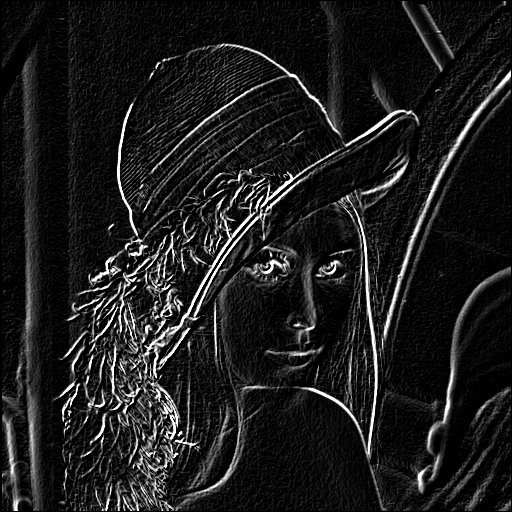
\includegraphics[scale=0.30]{sobelXY.jpg}
\caption{Resultado de aplicar el operador sobelXY para la imagen lena.jpg}
\end{figure}

\end{document} 
